\chapter{Realisation and Result}
This chapter describes the model, the architecture and the modules of MAELAB (Morphometric with Automatically Extraction of Landmarks) software. The first part is description about model as well as the packages in program. Then, we give the modules in program, class diagram and explain about it.
\section{Software architecture and the packages}
The MAELAB software mainly includes two packages: \textbf{MAgIS} package and \textbf{Morphometry} package. The \textbf{MAgIS} package contains the methods to segment images and construct the interface of program. This package was finished by NGUYEN Hoang Thao. The \textbf{Morphometry} package is the new one, it contains the implementations to estimate landmarks automatically. Besides, we also use the method provides by OpenCV library(OpenCV library) and Qt framework (Qt Framework package) (see in figure \ref{fig:42}).
\begin{figure}[h!]
\centering
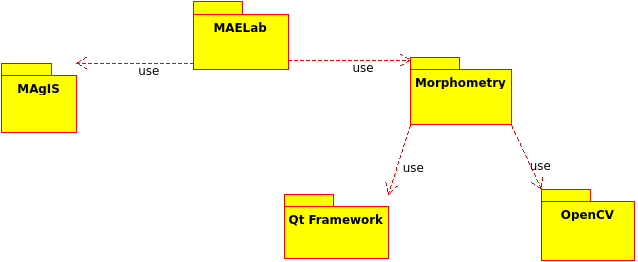
\includegraphics[width=0.8\textwidth]{./images/packages}
\caption{The packages of program}
\label{fig:42}
\end{figure}~\\
\section{The modules of software}
The software includes four main modules corresponding to four processes to estimate the landmarks: segmentation module, pairwise geometric histogram (PGH) module, probabilistic Hough transform (PHT) module and landmark detection module. Besides, the environment module provides the common classes. The classes in environment module can be used in all modules of software (figure \ref{fig:41}).
\begin{figure}[h!]
\centering
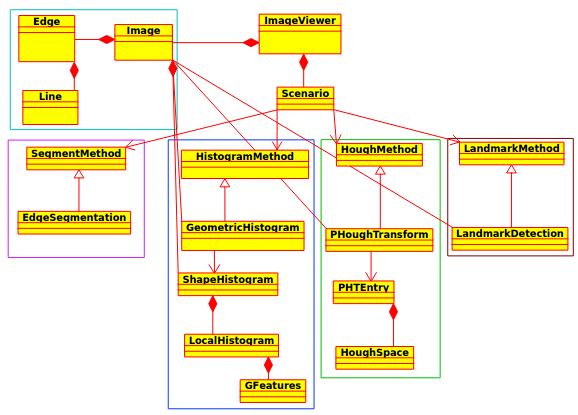
\includegraphics[width=0.8\textwidth]{./images/modules}
\caption{The modules of program with main classes}
\label{fig:41}
\end{figure}
\subsection*{Environment module}
Environment module contains the classes used to describe the information presented for object in image: \texttt{Image}, \texttt{Edge}, \texttt{Line}. The classes in this module can be used for all modules in MAELAB.
\begin{itemize}
\item The \texttt{Line} class descibes the information of a straight line and its method, such as: get the length of line, compute the perpendicular distance from a point to line, find the intersection between two lines, compute the angle between two lines, find the parallel line with this line.

\item The \texttt{Edge} class uses to present a curve and the methods with edge. An edge can be presented by a list of lines or a list of points. The important methods in \texttt{Edge} class are \texttt{breakEdge()} and \texttt{segment()} method. It used to break the edge into approximate lines based on the list of point constructed edge.

\item The \texttt{Image} class presents the information of an image such as file name, list of edge extracted from it. Besides, \texttt{Image} class also provides the methods to get the file name of image, compute the histogram of image, get the PGH of image, read its landmarks from a file, etc.
\end{itemize}
\subsection{Segmentation module}
The segmentation module implements the pre-process image and extracts the edges from image. The main classes in this module includes \texttt{SegmentMethod} class and \texttt{EdgeSegmentation} class. \texttt{SegmentMethod} class is designed as an abstract class of segmentation, this is the connecting port between this module and other modules. Class \texttt{EdgeSegmentation} extends from \texttt{SegmentMethod}, it implements the method to pre-process and extract the features from image by using the support methods from the \textit{environment} classes. Besides, \texttt{EdgeSegmentation} class also provide the access methods for other classes. The methods in \texttt{Edge segmentation} includes:
\begin{itemize}
\item Extract the approximate lines of object in an image,
\item Extract the approximate lines of object in each image in a folder.
\end{itemize}
\subsection{PGH module}
The PGH module provides the ways to implement the constructor of PGH and compute the measure metric between PGHs. In PGH module, class \texttt{HistogramMethod} is a abstract class, it provides the method to construct the PGH of an image. Its methods was implemented in \texttt{GeometricHistogram} class (\texttt{GeometricHistogram} extends from \texttt{HistogramMethod}). Basically, the method to construct the PGH come from other classes. Class \texttt{GeometricHistogram} uses these methods to finish the implementation from abstract class. In addition, \texttt{GeometricHistogram} also provides different methods in PGH such as: compute the measure metric by Bhattacharya metric, Chi-squared metric or Intersection metric; change the accuracy of PGH.\\
In detail, the classes used to construct the PGH and compare the measurement of them includes:
\begin{itemize}
\item \texttt{GFeatures} class contains the relative information of the objects in PGH such as angle, minimum distance and maximum distance. It provides the methods to get and set the relative information.

\item \texttt{LocalHistogram} class is constructed to contain the information when computing the PGH of a line in object. The chosen lines as reference lines, the local histogram is constructed based on recording the relating between reference line and other lines in object. Besides, it has the methods for the user to change the accuracy, such as the angle accuracy or the distance accuracy.

\item \texttt{ShapeHistogram} class constructs the PGH for an object. It is constructed by on combing all PGH of the lines in an object. It also provides the methods to compute the measured distance between the pairwise geometric histograms by a matching method. The methods in this class includes:
\begin{itemize}
\item Construct the PGH for an image,
\item Construct the matrix to save the PGH result,
\item Compute the measured distance between the two PGHs based on \textit{Bhattacharyya}, \textit{Chi-Squared} or \textit{Intersection} metric.
\end{itemize}

\item \texttt{GeometricHistogram} class provides the access ways for other classes. By usign this class, user can compute the pairwise geometric histogram of an image and calculate the distance between the pairwise geometric histograms.
\end{itemize}
\subsection{PHT module}
PHT module finishes the works in estimation stage. The main methods of PHT module stay in \texttt{PHoughTransform} class. It is a class extended from \texttt{HoughTransform} class, an abstract class. Besides the method extends from abstract class, \texttt{PHoughTransform} also implements the methods when we apply the probabilistic Hough transform as described in previous chapters.\\
The classes use PHT to estimate the model image from a scene image as follow:
\begin{itemize}
\item \texttt{HoughSpace} class contains the information about the angle and distance from a line to a reference point. These information is recorded to construct the accumulator when we apply the Probabilistic Hough Transform.

\item \texttt{PHTEntry} class presents each entry when constructing the reference table in the training process. Each entry contains the pair of lines and its information about angle and distance to a reference point.

\item \texttt{PHoughTransform} class describes the main process when we apply the probabilistic hough transform to estimate the landmarks. It includes the methods to construct the reference table, find the reference point in scene image and estimate the landmarks. Besides, it also provides the methods to estimated the landmarks of an image on the directory of images.
\end{itemize}
\subsection{Landmark detection module}
The landmark detection module used to implement the methods to refine the estimated landmarks from estimation stage. It includes an abstract class, \texttt{LandmarkMethod}, and an implement class which extends from abstract class, \texttt{LandmarkDetection} class. \texttt{LandmarkDetection} class implements the methods to refine the estimated landmarks and compare the accuracy between the estimated landmarks and manual landmarks.

%%%%%%%%%%%%%%%%%%%%%%%%%%%%%%%%%%%%%%%%%%%%%%%%%%%%%%%%%%%%%%%%%%%%%%%%%%%%%%
\iffalse
The figure \ref{fig:43} shows class diagram of this software. The \textbf{main} methods located in the \texttt{ImageViewer} class, where contains all functions of the software and connects with the \textbf{MAgIS} package. The connecting between the software and the modules made via \texttt{Scenario} class. To represent the information of image, we use the classes: \texttt{Line}, \texttt{Edge}, \texttt{Image}. For each main modules in program, we have the abstract classes, implementation classes and the support classes. \\
\begin{figure}[h!]
\centering
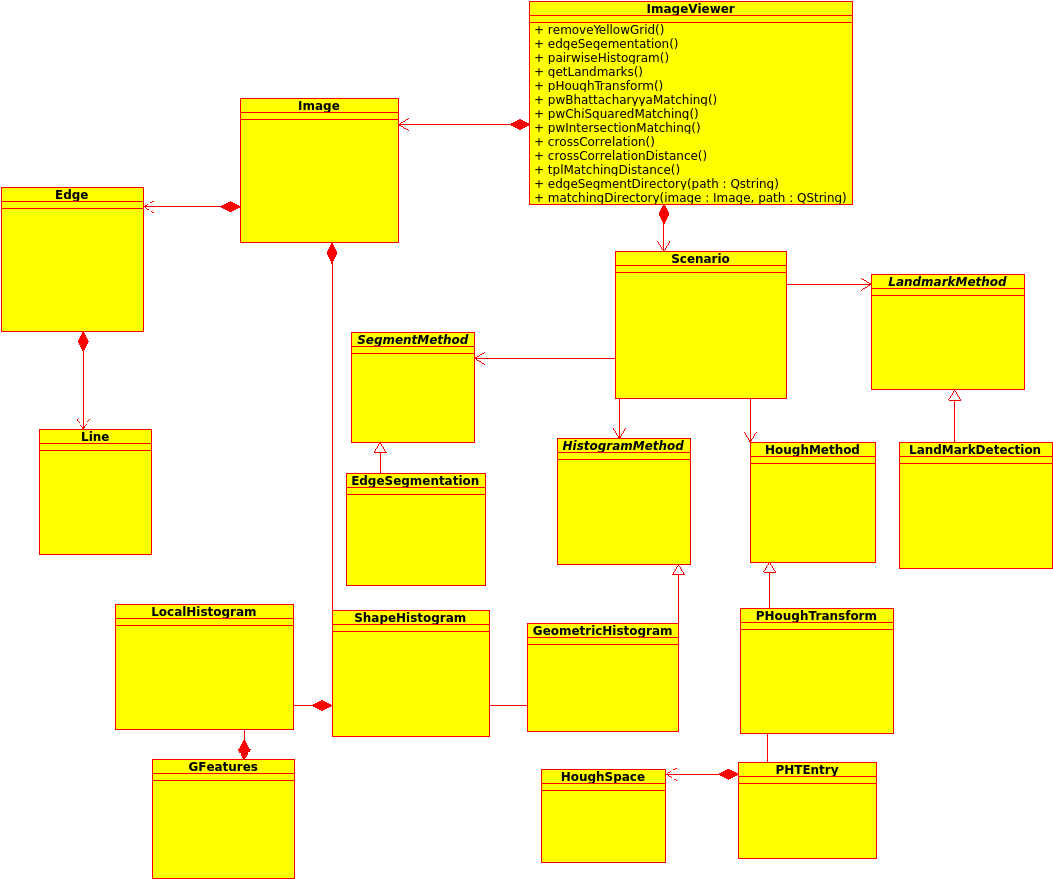
\includegraphics[width=1.1\textwidth]{./images/main}
\caption{The class diagram of program}
\label{fig:43}
\end{figure}
%%%%%%%%%%%%%%%%%%%%%%%%%%%%%%%%%%%%%%%%%%%%%%%%%%%%%%%%%%%%%%%%%%%%%%%%%%%%%%%%
\subsection*{The abstract classes}
The abstract classes contains the abstract methods correspondence with the main modules of program. They provide the abstract methods which was implemented in the inherit classes. As introduce in previous section, the abstract classes include: \texttt{HistogramMethod} class, \texttt{SegmentMethod} class, \texttt{HoughMethod} class, \texttt{LandmarkMethod} class.

\subsection{Pairwise Geometric Histogram}

\subsection{Estimate the global pose (Probabilistic Hough Transform)}

\subsection{Refine the landmarks}
\texttt{LandmarkDetection} class provides the methods to refine the estimated landmarks by probabilistic Hough transform. It also implements the cross-correlation technique to match the model and the image and provides the methods to compare the estimated result with the original result (by comparing distance between the landmarks).
\fi
%%%%%%%%%%%%%%%%%%%%%%%%%%%%%%%%%%%%%%%%%
\section{Result}
As presentation about our result, this section introduces about MAELAB software, the parameters used in execution and the discussion about the result. All these results have been obtained with the set of left mandibles and right mandibles of the beetle (each set includes 293 images).
\subsection{New interface}
All parts of the new code are integrated into MorphoEcol\footnote{Morphometry in Ecologie} software. To focus on the main functions available to compute landmarks, we reface the interface of program to dedicate the methods that we have presented (figure \ref{fig:44}).
\begin{figure}[h!]
\centering
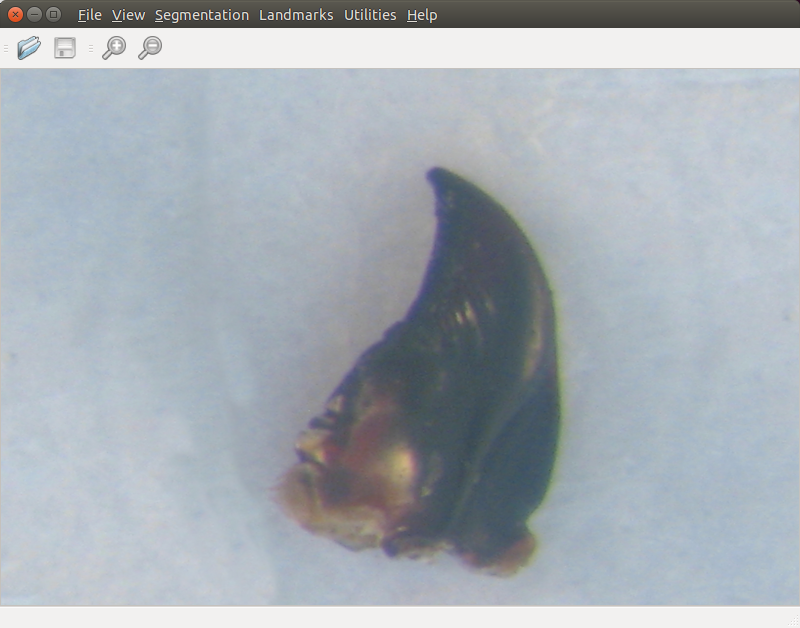
\includegraphics[width=0.7\textwidth]{./images/software}
\caption{The graphic user interface of MAELab software}
\label{fig:44}
\end{figure}~\\
In the new interface of program, the users can find the functions in MAELAB software are:
\begin{itemize}
\item Image segmentation by analysing histogram (in \textbf{Segmentation} menu)
\item Removing the yellow grid on image (in \textbf{Utilities} menu)
\item Loading the manual landmarks (in \textbf{Utilities} menu)
\item Computing the pairwise geometric histogram (PGH) of image (in \textbf{Utilities} menu)
\item Computing the measure metric between PGHs by Bhattacharya, Chi-Squared or Intersection method (in \textbf{Utilities} menu)
\end{itemize}
\begin{figure}[h!]
\centering
\subfloat[MAELab software]
{\label{fig:451}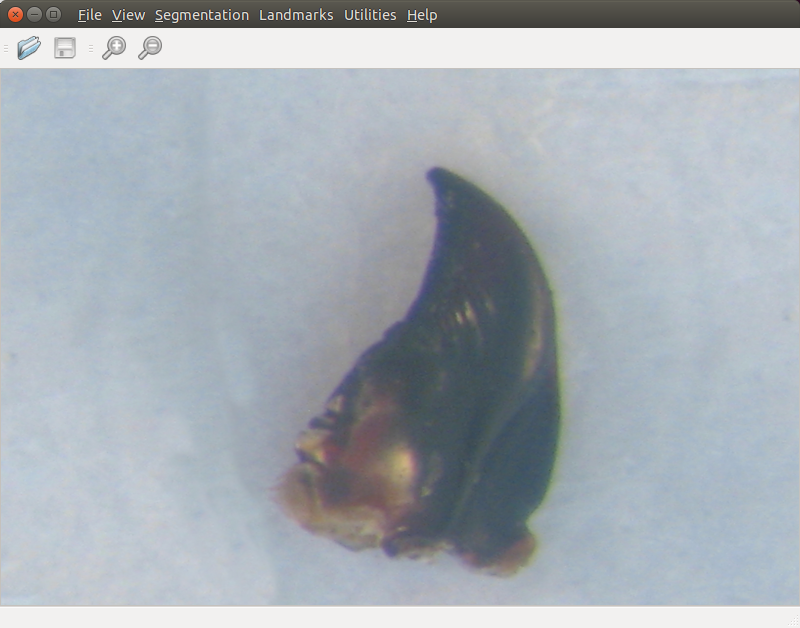
\includegraphics[width=0.45\textwidth]{./images/software}}~~
\subfloat[MAELab with Segmentation menu]
{\label{fig:452}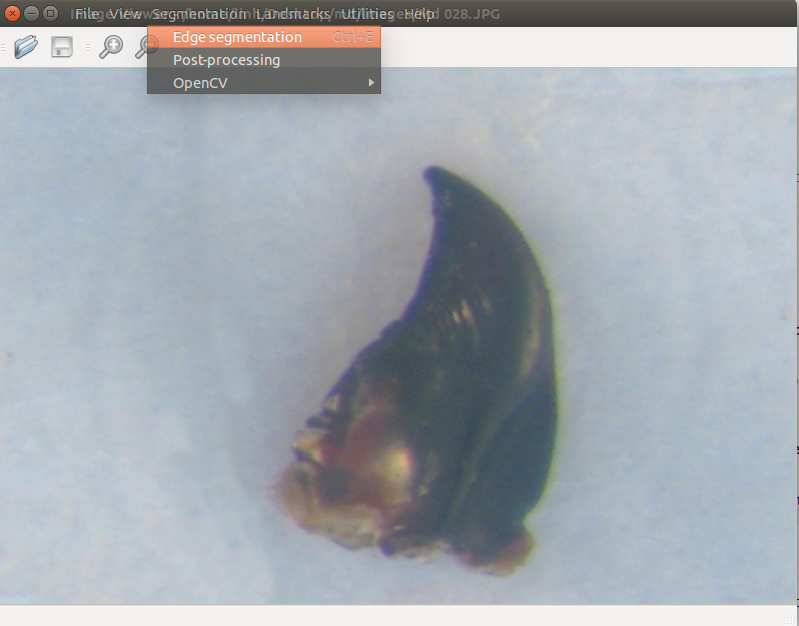
\includegraphics[width=0.45\textwidth]{./images/newiface1}}\\
\subfloat[MAELab with Landmarks menu]{\label{fig:453}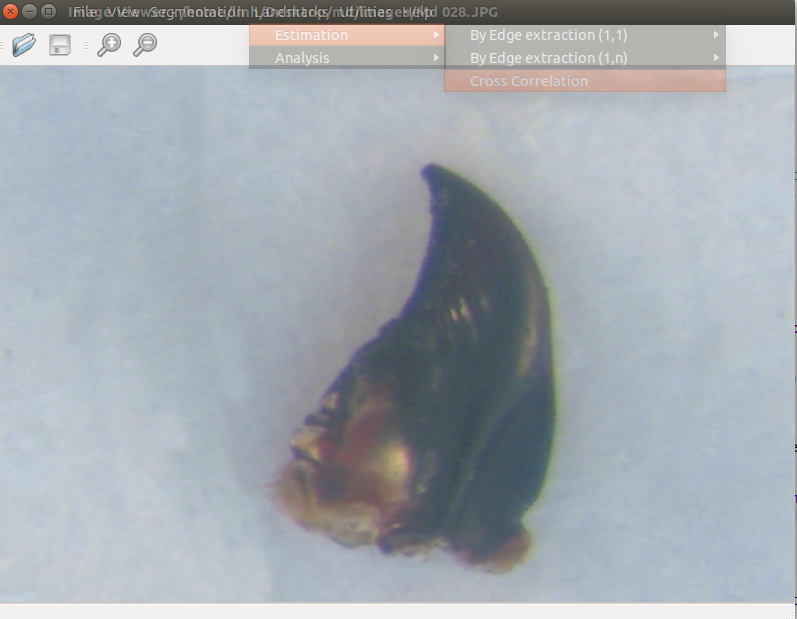
\includegraphics[width=0.45\textwidth]{./images/newiface2}}~~
\subfloat[MAELab with Utilities menu]
{\label{fig:454}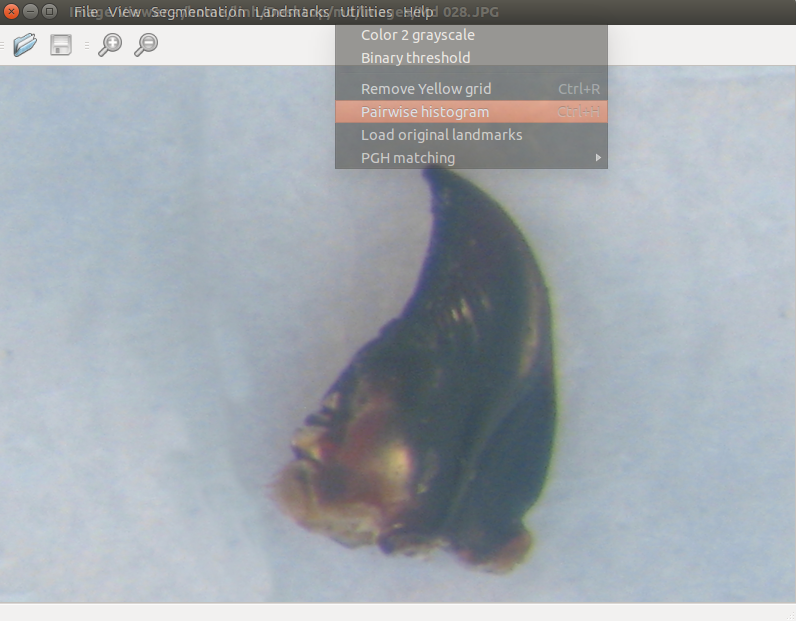
\includegraphics[width=0.45\textwidth]{./images/newiface3}}
\caption{The MAELab software with its menu}
\label{fig:45}
\end{figure}~\\[0.2cm]
\subsection{Experimentation}
The experimentation is deployed on two machines with difference equipment:
\begin{itemize}
\item Machine 1: Intel(R) Core(TM) 2 Duo CPU T8100 2.1GHz, 2 GB of RAM
\item Machine 2: Intel(R) Core(TM) i7-4790 CPU 3.6GHz, 16 GB of RAM
\end{itemize}
The testing data is two set of biological images: \textit{Right mandible and left mandible}. Each dataset includes 293 images(3264 x 2448). However, the data was filtered by suppressing the bad images in the both datasets. The bad images includes the empty images and broken images (images contain the broken object). They are showed as below:
\begin{multicols}{3}
\begin{itemize}
\item Md 004.JPG
\item Md 146.JPG
\item Md 238.JPG
\item Mg 003.JPG
\item Mg 007.JPG
\item Mg 040.JPG
\item Mg 066.JPG
\item Mg 159.JPG
\item Mg 248.JPG
\item Mg 292.JPG
\end{itemize} 
\end{multicols}
Because the estimation method has several steps, we decide focus on some steps of method, such as segmentation and estimation. For each step, we compute the execution time on one image and a list of images. Then we compare the runtime between two examination systems (see in table \ref{table_runtime1} and table \ref{table_runtime2}).

Machine 1:
\begin{table}[h]
	\centering
	\begin{tabular}{|c|c|c|}
		\hline
		No of images & Segmentation(second) & Estimation(second) \\ \hline
		1 & 0.844 & 31.4245   \\ \hline
		290 & 571.576 & 13000.9131   \\ \hline
	\end{tabular}	
	\caption{The runtime of program on machine 1}		
	\label{table_runtime1}
\end{table}

Machine 2:
\begin{table}[h]
	\centering
	\begin{tabular}{|c|c|c|}
		\hline
		No of images & Segmentation(second) & Estimation(second) \\ \hline
		1 & 0.27782 & 10.4392   \\ \hline
		286 & 171.589 & 4665.79   \\ \hline
	\end{tabular}
	\caption{The runtime of program on machine 2}
	\label{table_runtime2}
\end{table}
Based on the runtime tables, the most of runtime stays in stage of estimation. This is the time to execute two steps: estimated landmarks (by PHT) and refine landmarks (by template matching). Hence, it also depend on the configuration of system.
\subsection{Parameters}
In our program, we use these parameters for the methods:
\begin{itemize}
\item The best segmentation obtained from choosing a good threshold value. In the program, Canny algorithm is applied to segment the image. Thus, the ratio between \textit{lower threshold : upper threshold} is important to get a good result. And the ratio is: \textit{1 : 3} (in class \texttt{Image}, method \texttt{getEdges}), this ratio has been chosen experimentally. The lower value is 1 * \textit{threshold} value and the upper value is 3 * \textit{threshold} value. The \textit{threshold} value is identified by analysing the histogram of image. 
\item The angle and distance accuracy used in constructing the PGH matrix and calculate the measure distance between PGHs. The angle accuracy can be 90 (0.5 * 180), 180, 360 (2 * 180), 720(4 * 180), 1080(6 * 180), 2160(12 * 180) degree. The distance accuracy can be 250, 500 or 1000 columns. The \textbf{default value} in program is \textbf{180} degree for angle accuracy, and \textbf{250} for the distance accuracy. 
\item During applying the Probabilistic Hough Transform, to reduce the time complexity during training, we consider the pair of closet lines. And the parameters used to indicate the closet line are (used in method \texttt{closetLine}, class \texttt{PHoughTransform} ):
	\begin{itemize}
		\item Length of each line greater than \textbf{60} pixels
		\item Angle between two lines greater than \textbf{15} degree
		\item Perpendicular distance from one of two endpoints of a line to other line less than \textbf{5} pixel.
	\end{itemize}
The conditions to predicate two pairs of lines are similar (used in method \texttt{similarPairLines}, class \texttt{PHoughTransform}):
	\begin{itemize}
		\item Subtraction between angle of two pair of lines is less than \textbf{1}
		\item Subtraction between ratio couple of scene lines and reference lines is less than \textbf{1}
		\item Subtraction between distance of two pair of lines is less than \textbf{2}
	\end{itemize}
\item The size of bounding box around the reference landmarks used for estimating landmarks by cross-correlation method or computes the estimated centroid is \textit{400} pixels (used in method \texttt{crossCorrelation and crossCorrelationDistance}, class \texttt{ImageViewer})
\item The size of bounding box around reference landmarks and estimated landmarks used to refine the estimated landmarks or compute the estimated centroid are \textit{400} pixels and \textbf{1400} pixels, respective.(used in method \texttt{getLandmarks and tplMatchingDistance}, class \texttt{ImageViewer})
To increase the flexible of program, all parameters was placed in the resources files (\textbf{data/resources} folder). For each group of parameters, the parameters are put in a file.
\end{itemize}
\subsection{Results}
The automated landmark identification is examined on two data sets: \textit{right mandible and left mandible}. And the landmarks are extracted: 18 landmarks for each \textit{right mandible} image, 16 landmarks for each \textit{left mandible} image.\\
\begin{figure}[h!]
\centering
\subfloat[The scene image]{\label{fig:461}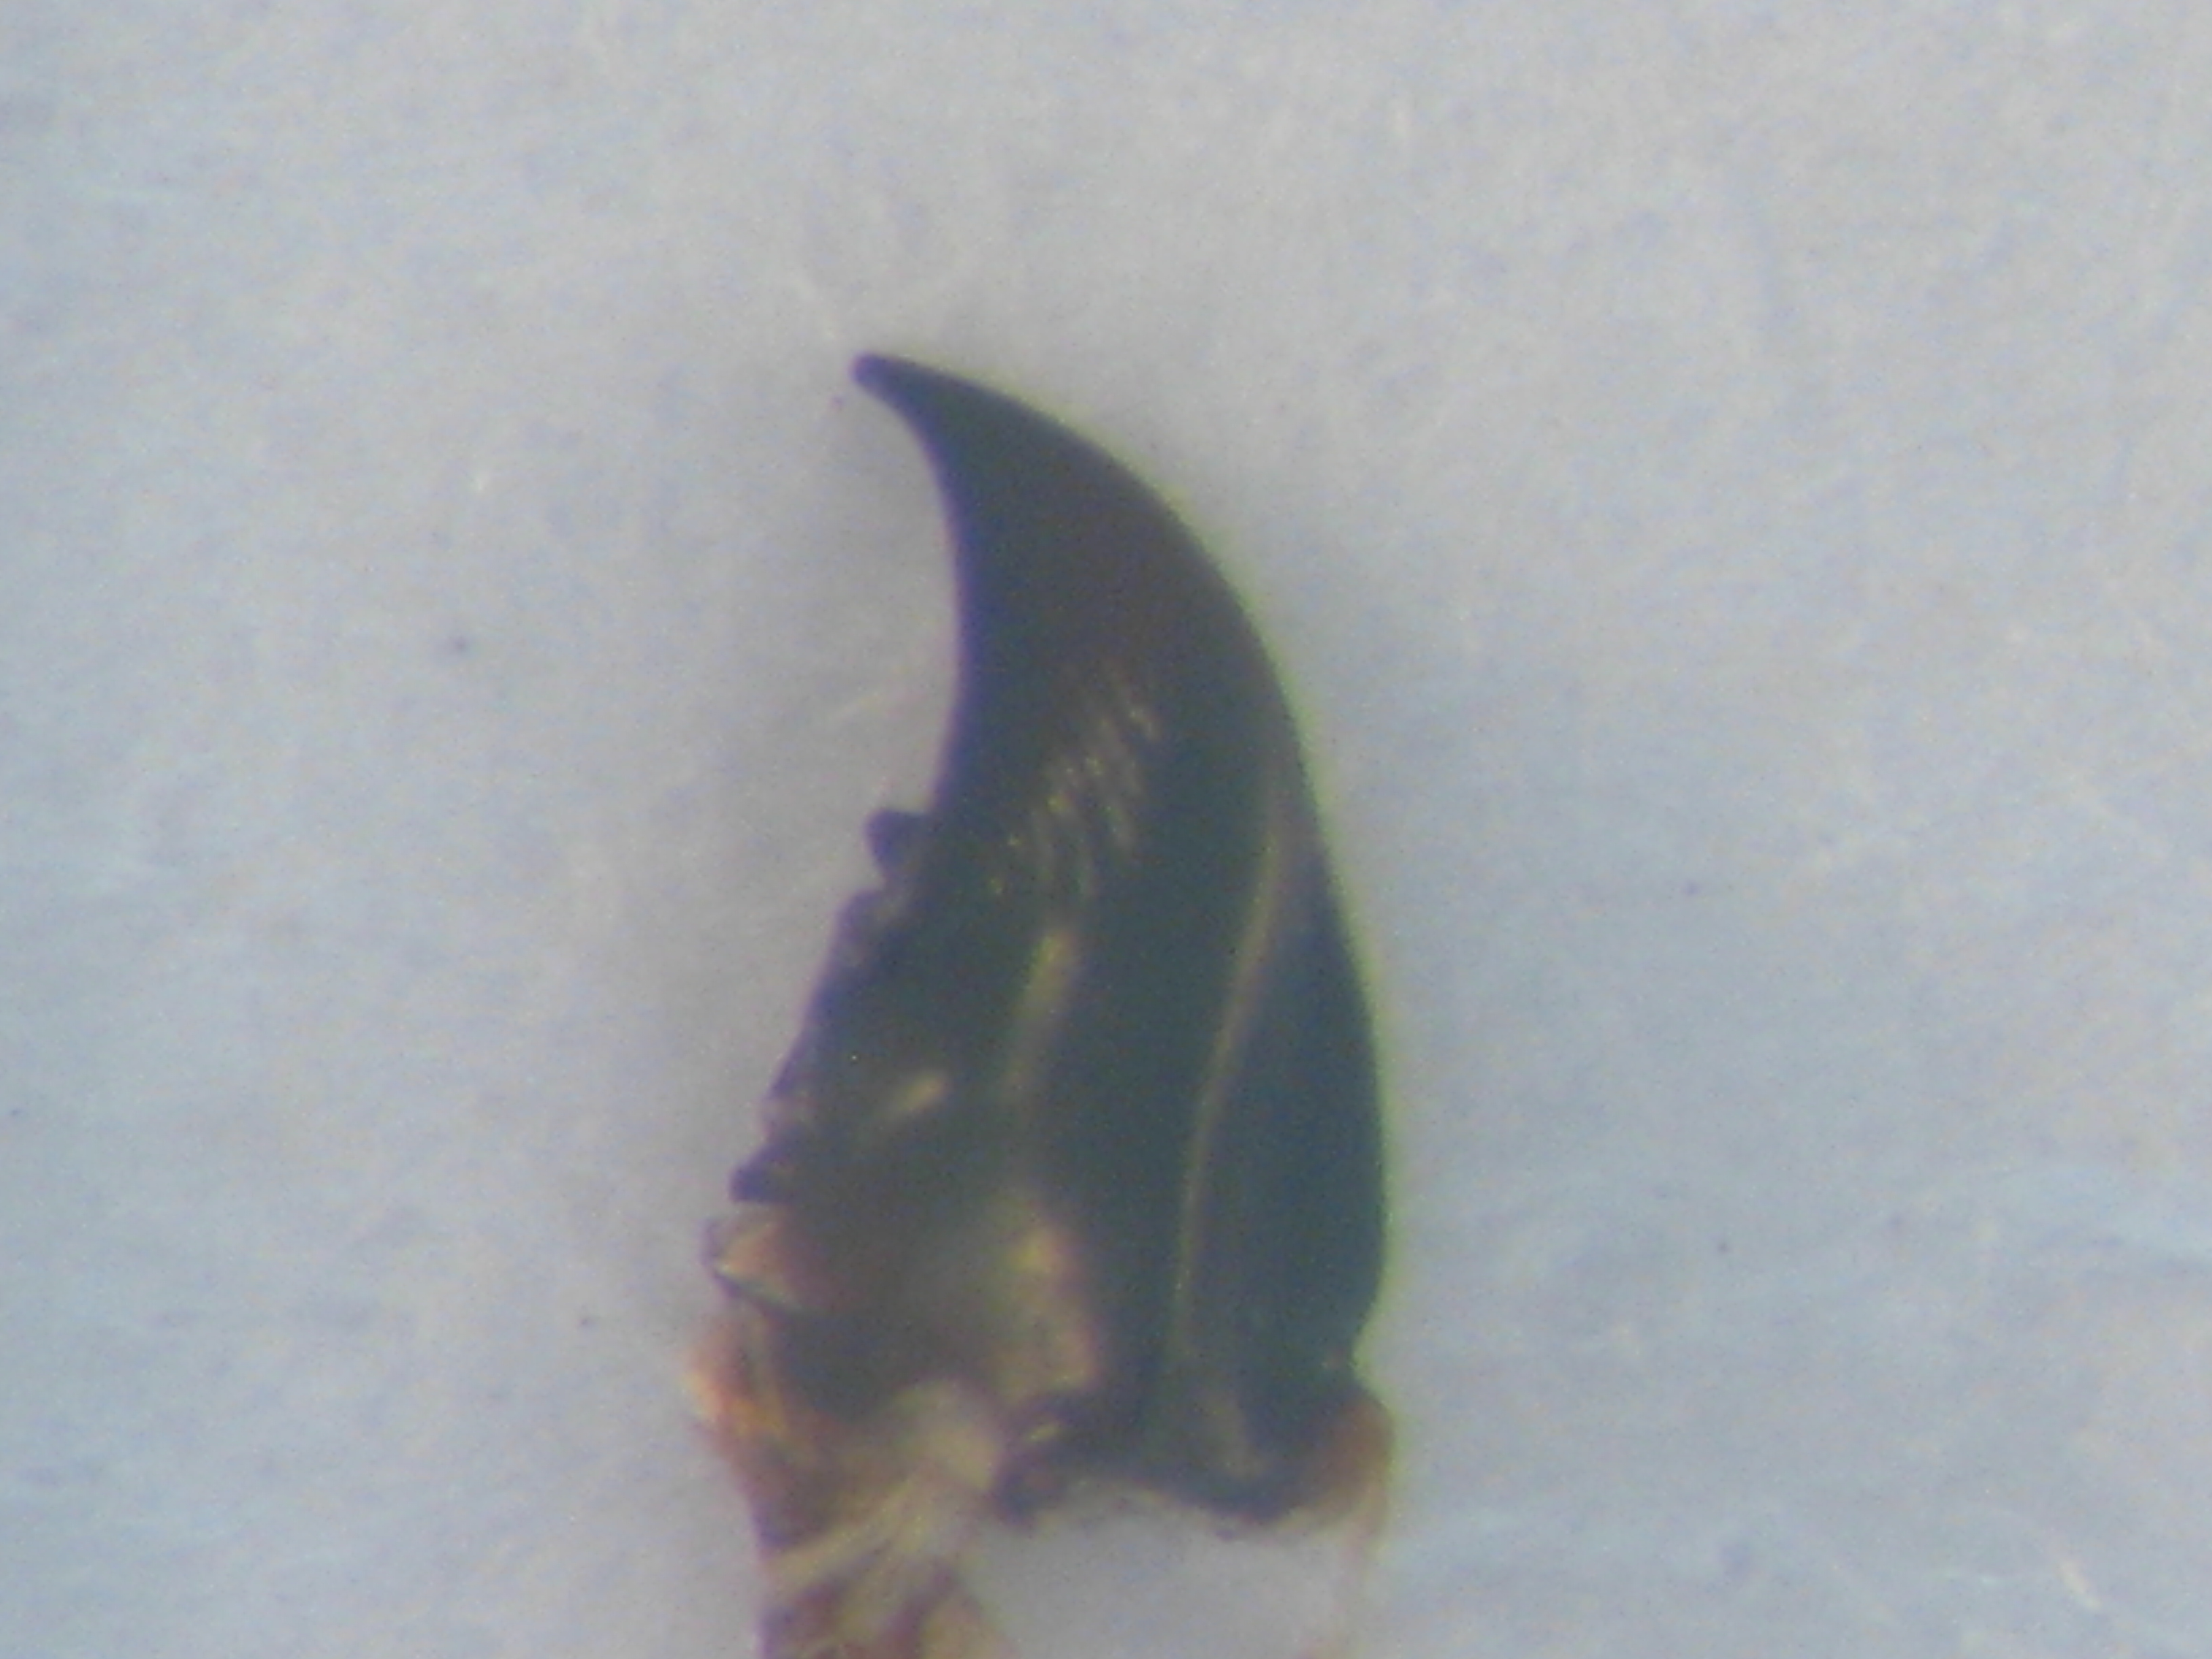
\includegraphics[width=0.45\textwidth]{./images/md32}}\\
\subfloat[The scene image with estimated landmarks by cross-correlation ]{\label{fig:462}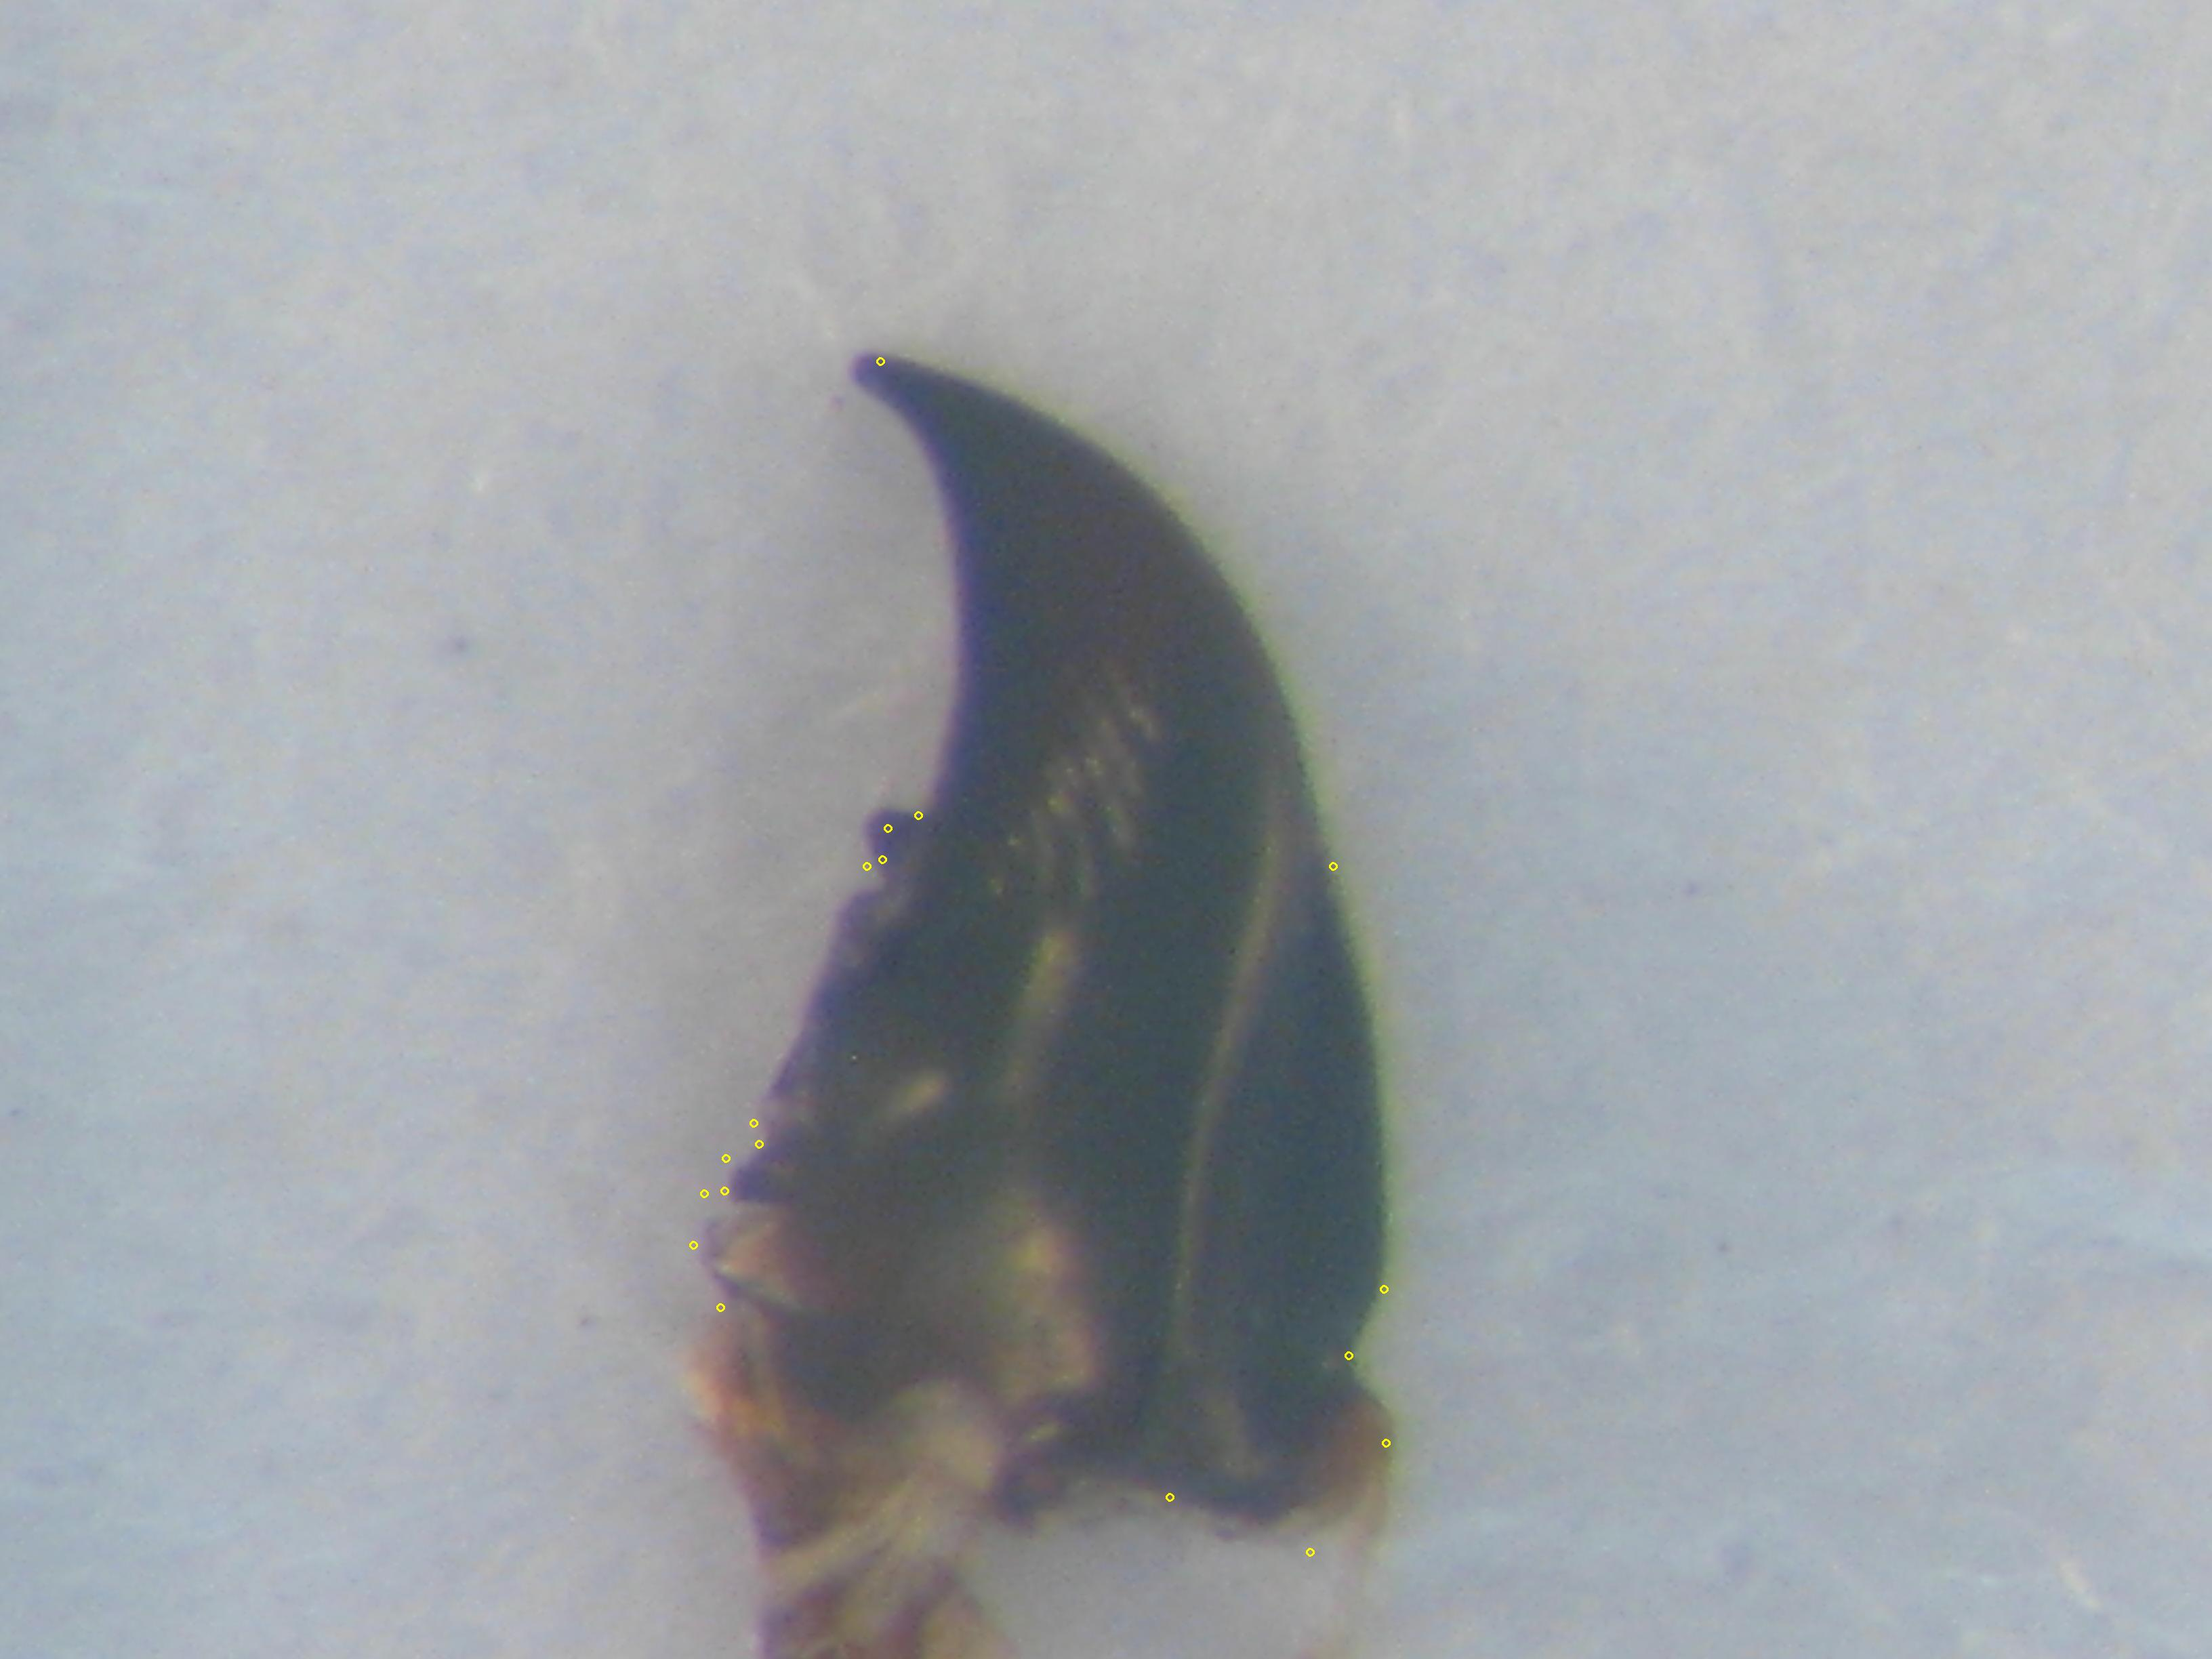
\includegraphics[width=0.45\textwidth]{./images/md32_cross}}~~
\subfloat[The scene image with estimated landmarks (by article) ]{\label{fig:463}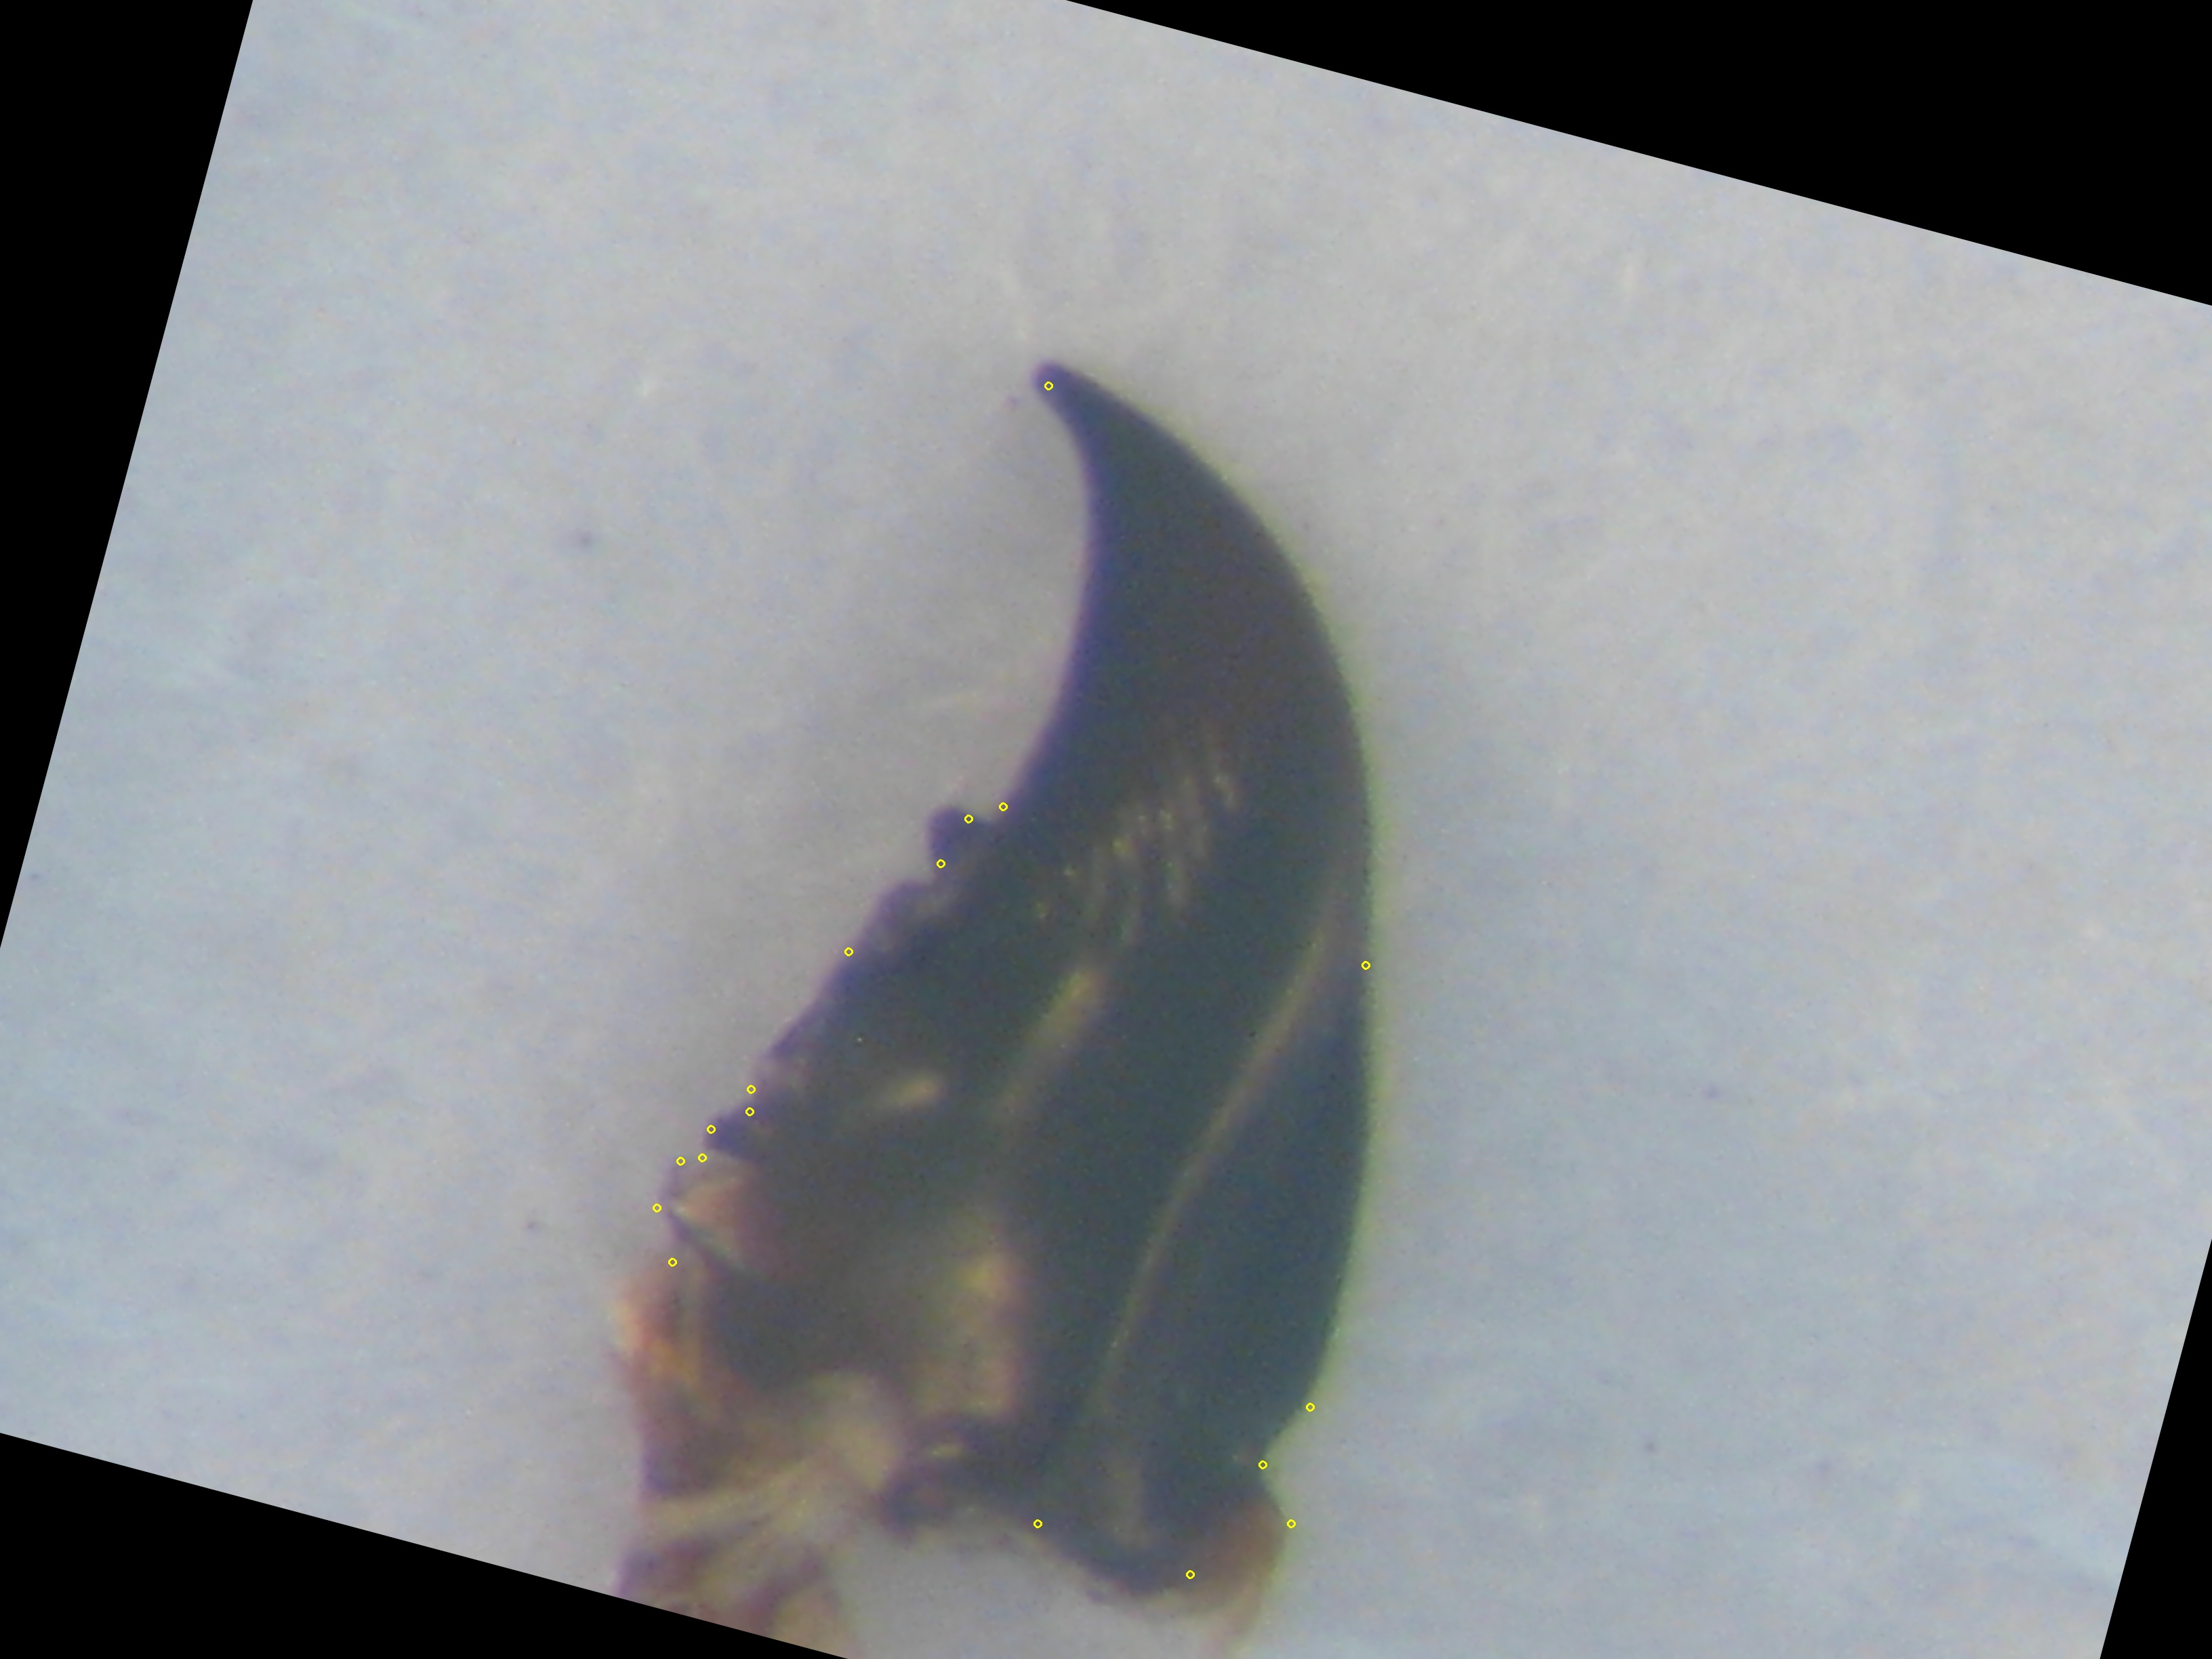
\includegraphics[width=0.45\textwidth]{./images/est32}}
\caption{Automatic identification of the landmarks}
\label{fig:46}
\end{figure}~\\
To have the basic evaluation about this method, we compare its result with the result from \textbf{``original"} of cross-correlation method. Obvious, the location of landmarks obtained from method (follows article) more closer than the landmarks obtained from cross-correlation (see in figure \ref{fig:46}).\\
Besides, the accuracy of the system can be determined by comparing the differences(in pixels) between the landmarks located by this method and the manual landmarks. This method has to pass several steps, the result of each step will effect on next steps. Thus, to evaluate the accuracy of this method, we can evaluate the result of each step.
\subsection{Limits and future works}
The method includes several steps to get the last result. At each step, we can use different ways to do. The methods proposed in this report just a part of them. Moreover, the program has use the parameters as the conditions, changing the values of parameters can effected to the accuracy of program.
Currently, the work finishes on two sets of data: \textit{right mandible} and \textit{left mandible}. In the future, we can evaluate and improve this method. Then applying this method on other dataset of biological images.